% //TODO:真空ポンプを用いた場合と電磁石を用いた把持方法の比較文章を書く
\section{実験装置の改良による影響に関して}
\label{sec:reexp}

先行研究\cite{ref:8}において,電磁石を用いて,磁力によって球の把持を行っていた.一方で,本研究において,強磁性体以外の球の把持を行うため,真空ポンプを用いて吸引する手法に変更した.その把持手法の変化に伴う影響を議論する.

% Fig.\ref{fig:re-exp-vaccume}に真空ポンプを用いた把持方法における再現性の確認の実験結果を示す.縦軸は落下速度,横軸は落下開始時からの経過時間である.この再現性確認において,溶液の再作成から行った.終端速度に達するまでの経過はほぼ同様であった.一方で,終端速度は約10\%の誤差が生じた.これは,溶液の作製による誤差の影響を受けていると考えられる.

% \begin{figure}[ht]
%     \centering
%     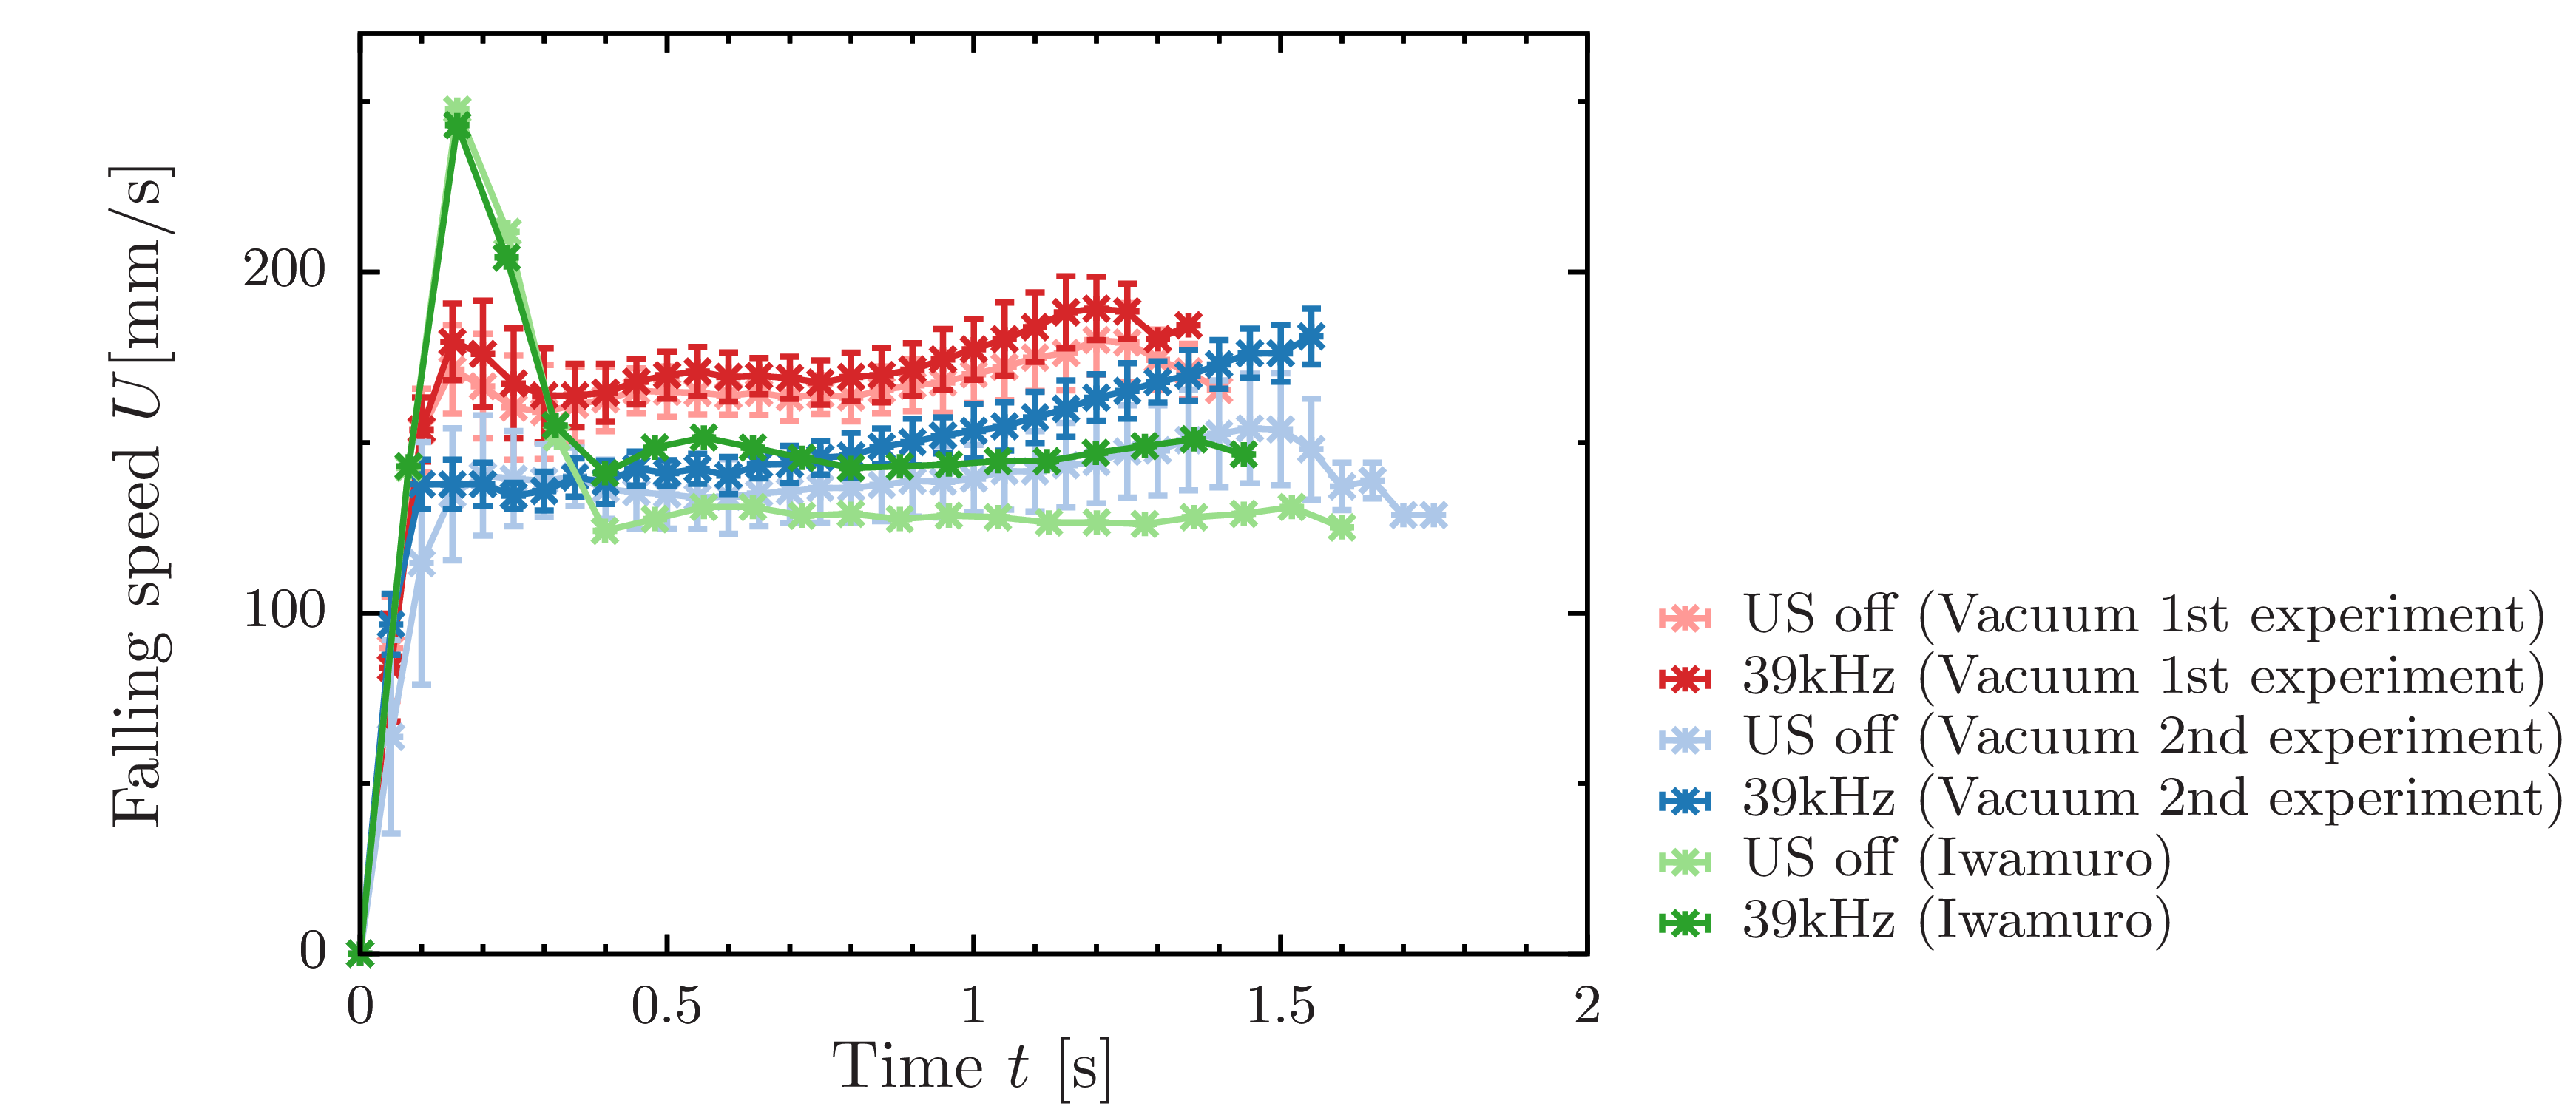
\includegraphics[width=14cm,clip]{X-Appendix/reexp.png}
%     \caption{Falling velocity of a sphere in 1wt.\%PAA solution with and without ultrasound irradiation in tank A (reproducibility check).}
%     \label{fig:re-exp-vaccume}
% \end{figure}

\subsection{落下実験結果}

容器Aにおいて,真空ポンプを用いて球を落下させた.解析した結果をFig\ref{fig:falling-A}に示す.縦軸は落下速度,横軸は落下開始時からの経過時間である.先行研究であるIwamuro \textit{et al}.\cite{ref:8}や電磁石を用いて球を把持した場合と比較し,超音波照射による高速化が顕著に現れていないことが分かる.また,落下開始時に電磁石を用いた場合はオーバーシュートが見られるが,真空ポンプを用いた場合はオーバーシュートが見られなかった.このことに関して,後述の第\ref{sec:dis-de}節にて議論を行う.また,補足資料\ref{sec:reexp}に真空ポンプを用いた把持方法における再現性の確認結果を示す.

\begin{figure}[ht]
    \centering
    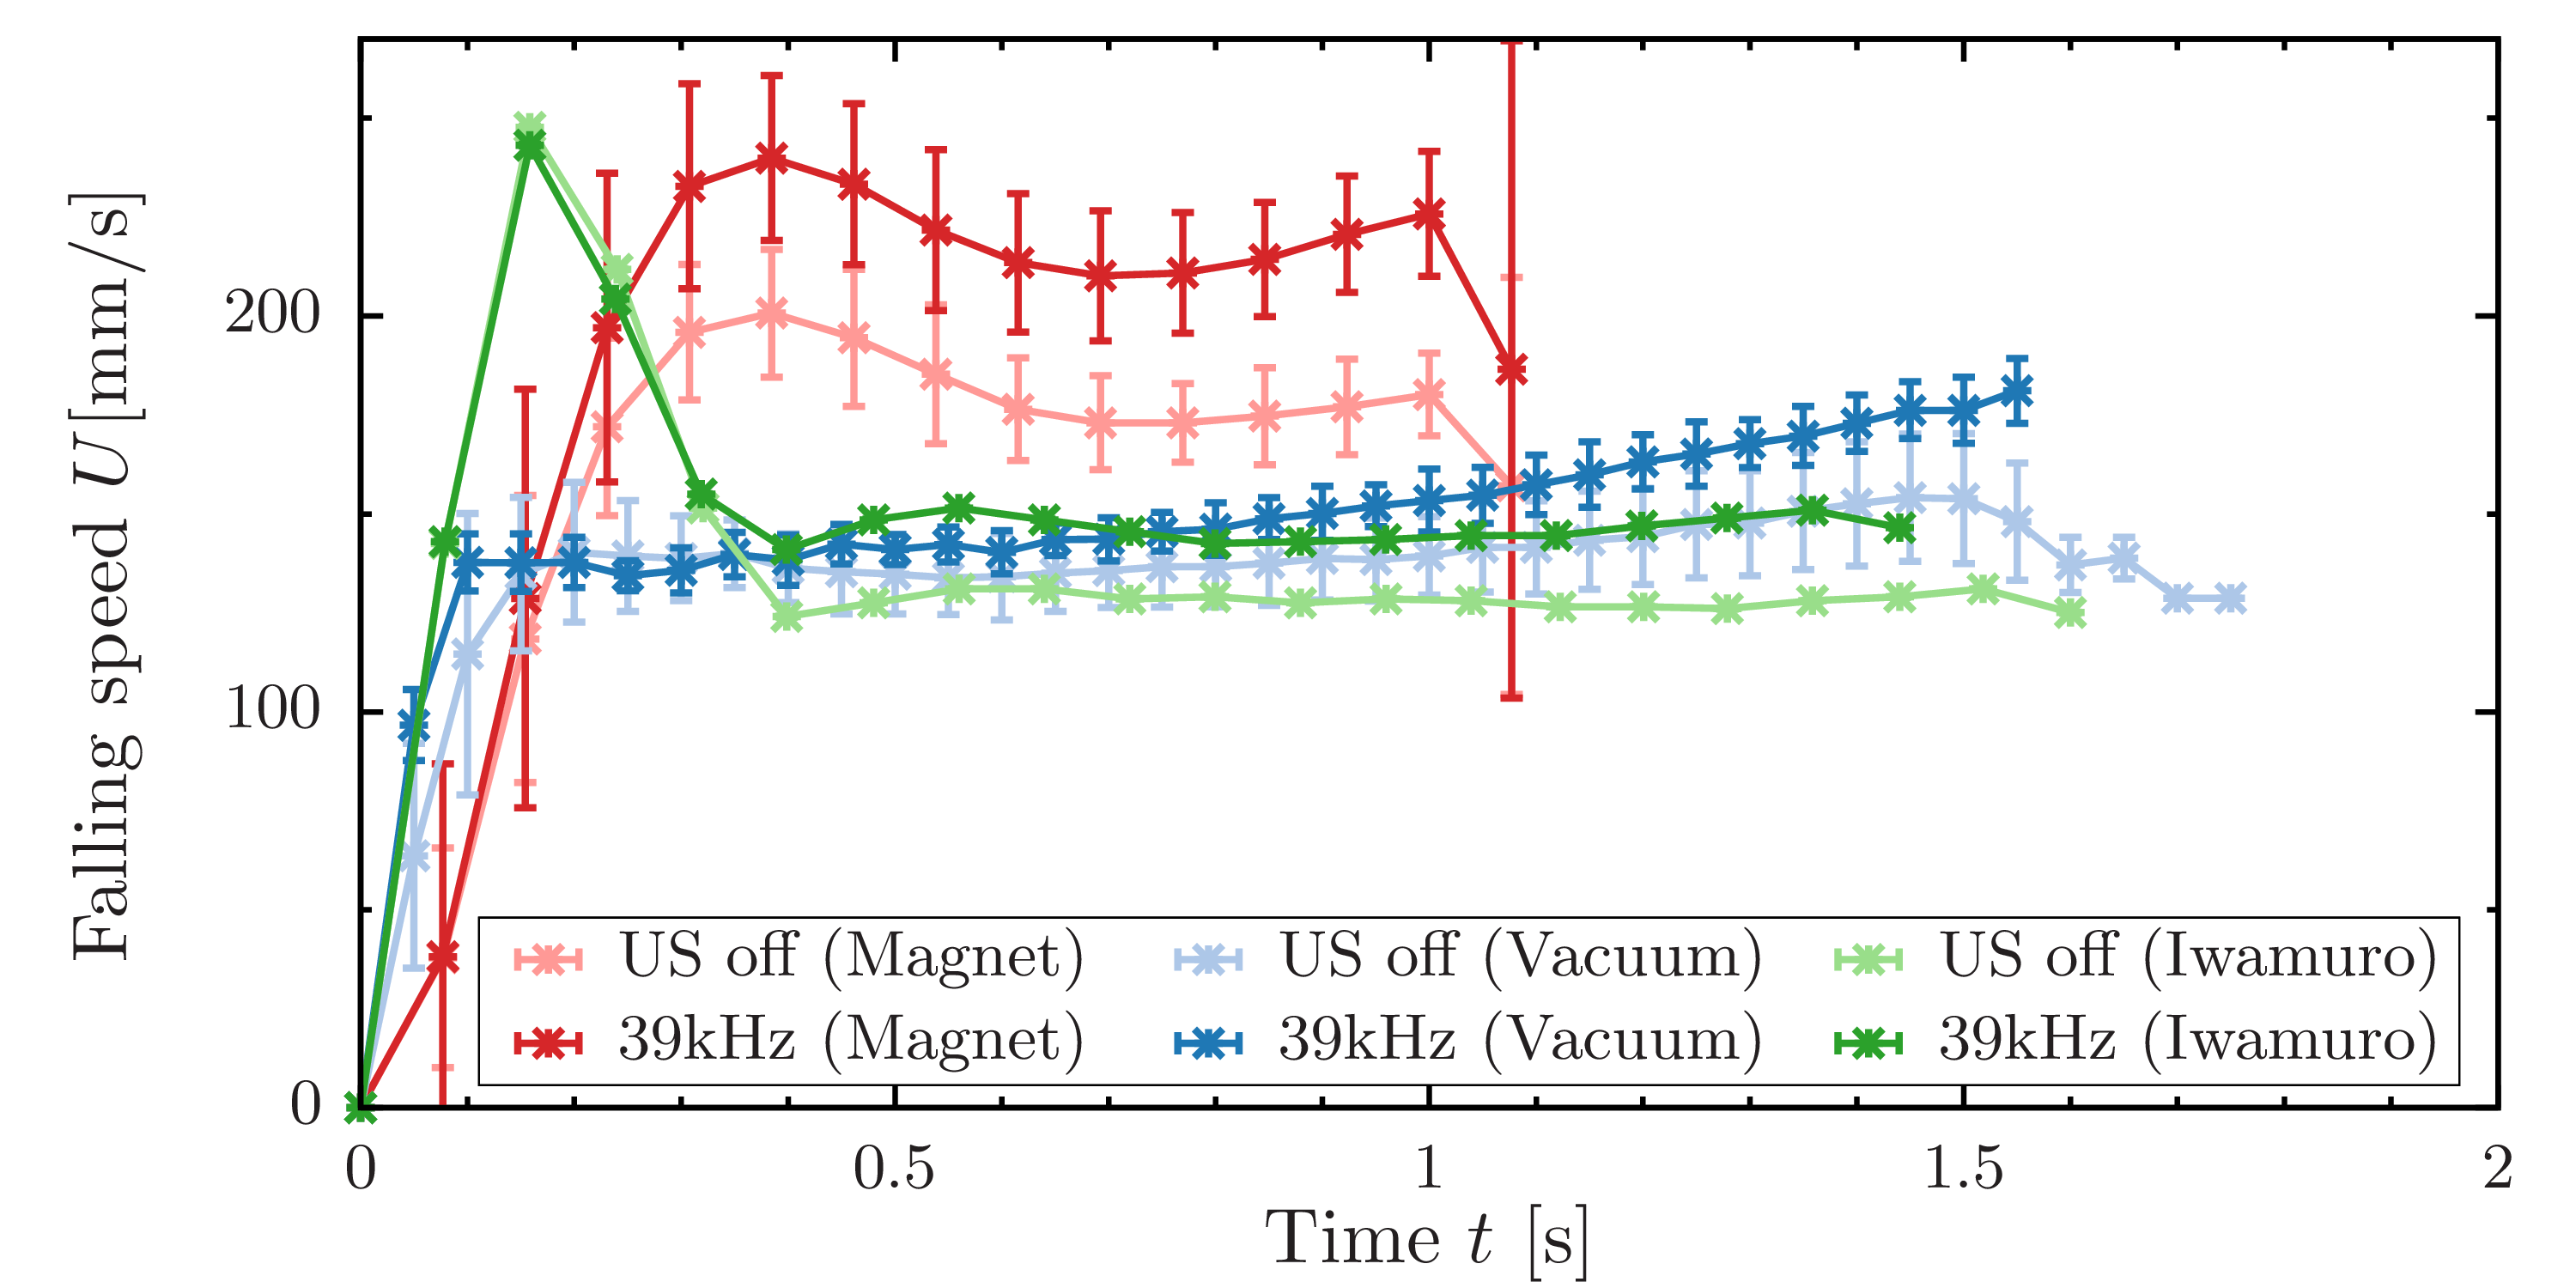
\includegraphics[width=12cm,clip]{./5-Results/s1-A.png}
    \caption{Falling speed of a sphere in 1wt.\%PAA solution with and without ultrasound irradiation in tank A.}
    \label{fig:falling-A}
\end{figure}

\subsection{実験装置改良に伴う終端速度の変化}

上記の式(\ref{eq:UT})より,Power-Law modelにおける,$k$,$n$のパラメータより終端速度を見積もることができる.

Table \ref{table:power-law}の結果より,式(\ref{eq:UT})を用いて直径10mmの球におけるIwamuro\cite{ref:8}の終端速度$U_I$を基準とした終端速度の比$U_T/U_{I}$を求めた.その結果を,Table \ref{table:UT}に示す.これより,今回の粘度特性において,Iwamuro\cite{ref:8}と比較して終端速度が1.09倍速くなることが分かった.Fig.\ref{fig:falling-A}において,Iwamuro\cite{ref:8}と比較して1.125倍,終端速度が速かった.一方で,0.95,1.05wt.\%それぞれのPAA溶液の粘度特性における終端速度比と比較しても実験結果と一番近いのは,1wt.\%の場合である.よって,溶液の濃度精度は1wt.\%±0.05wt.\%以内であり,溶液の作製誤差によって落下速度に差が生じたと考えられる.

\begin{table}[h]
    \centering
    \caption{Each parameter($k$,$n$) and terminal speed ratio in the power-law model for each experimental result.}
    \label{table:UT}
    \begin{tabular}{c|c|c|c} \hline
                                                     & $k$  & $n$  & $U_T/U_{I}$ \\ \hline \hline
        Present Value(1.05wt.\%)                     & 9.56 & 0.23 & 0.93        \\
        Present Value(1wt.\%)                        & 8.37 & 0.24 & 1.09        \\
        Present Value(0.95wt.\%)                     & 5.22 & 0.25 & 3.91        \\
        Iwamuro\cite{ref:8}                          & 9.4  & 0.23 & 1           \\
        Shiratori \textit{et al}.(2016)\cite{ref:10} & 5.9  & 0.25 & 2.99        \\ \hline
    \end{tabular}
\end{table}

\newpage

\subsection{落下開始時のオーバーシュートへの影響}
\label{sec:dis-de}

今回,球を把持する手法を,電磁石を用いて把持する方法から真空ポンプを用いて把持する方法に変化させた.この時,落下開始時0-0.3sにおける落下速度のオーバーシュートが,先行研究\cite{ref:8,ref:9}より小さくなった.落下開始時のオーバーシュートは弾性による影響によって生じる\cite{ref:12}.以下で,オーバーシュートが見られなくなった原因を,物質の流動性を表す$De$数より考える.$De$数が大きくなると,弾性的傾向が強くなり,$De$数が小さくなると,粘性的流動を表す.

$De$数は下記の様に緩和時間$\lambda$[s],代表時間$T$[s]の比で表される.
\begin{equation}
    De = \frac{\lambda}{T} .
    \label{eq:De}
\end{equation}
代表時間$T$[s]に関して,超音波照射を行っていない場合の球の落下条件においても考えるため,
\begin{equation}
    T = \frac{a}{U} ,
    \label{eq:T}
\end{equation}
となる.ここで,球の落下速度$U$[m/s],球の半径$a$[m]である.また,緩和時間$\lambda$[s]は,
\begin{equation}
    \lambda \approx \frac{\mu}{G'} .
    \label{eq:lamda}
\end{equation}
ここで粘度$\mu$[Pa$\times$s],貯蔵弾性率$G'$[Pa]である.緩和時間は変形の経過時間において,粘弾性流体が流体的挙動を示すか,固体的挙動を示すかの指標である\cite{ref:sakanishi}.粘度$\mu$[Pa$\times$s]に関して,せん断速度$\dot{\gamma}$[1/s]および粘度定数$k$[Pa$\times$s${}^n$],指数$n$を用いてPower-law modelに従うとすると,
\begin{equation}
    \mu = k \times \dot{\gamma}^{n-1} ,
    \label{eq:power-law}
\end{equation}
となる.落下球によるせん断領域において,せん断速度の代表値$\dot{\gamma}$[1/s]は,次のように概算される.
\begin{equation}
    \dot{\gamma} \sim \frac{U}{a} .
    \label{eq:gamma}
\end{equation}
よって,式(\ref{eq:power-law}),(\ref{eq:gamma})よりせん断領域における粘度$\mu_U$は,次式で概算される.
\begin{equation}
    \mu_U \sim k \times \left(\frac{U}{a}\right)^{n-1} .
    \label{eq:power-law2}
\end{equation}
これら式(\ref{eq:De}),(\ref{eq:T}),(\ref{eq:lamda}),(\ref{eq:power-law2})より,$De$数は,
\begin{equation}
    De \sim \frac{k}{G'} {\left(\frac{U}{a}\right)}^n ,
    \label{eq:De2}
\end{equation}
となり,粘度定数$k$[Pa$\times$s${}^n$],貯蔵弾性率$G'$[Pa],落下速度$U$[m/s],球の半径$a$[m]によって表される.

貯蔵弾性率$G'$[Pa]に関して,先行研究において計測されたFig.\ref{fig:iwamuro-G}(b)の結果より考える.この図において,貯蔵弾性率$G'$[Pa]は応力$\tau$[Pa]との関係性が示されている.ここで応力$\tau$[Pa]は,
\begin{equation}
    \tau = \mu \times \dot{\gamma} ,
    \label{eq:tau}
\end{equation}
となる.ここに,式(\ref{eq:power-law}),(\ref{eq:gamma})を代入すると,
\begin{equation}
    \tau \sim k \times \left(\frac{U}{a}\right)^n ,
    \label{eq:tau-cal}
\end{equation}
と概算することができる.

Fig.\ref{fig:falling-A}, \ref{fig:iwamuro-fall}それぞれの結果より,ピーク速度$U_{peak}$[mm/s]と終端速度$U_{ave}$[mm/s]を算出した.続いて,式(\ref{eq:tau-cal})を用いて,それぞれの速度における応力$\tau_{peak}$[Pa],$\tau_{ave}$[Pa]の算出を行った.これら算出結果と先行研究の計測結果Fig.\ref{fig:iwamuro-G}より,貯蔵弾性率$G'$も求めた.これらの結果を,Table \ref{table:iwamuro}に示す.

また,式(\ref{eq:power-law2})を用いて,ピーク速度/終端速度それぞれの粘度$\mu_{peak}$[Pa$\cdot$s],$\mu_{ave}$[Pa$\cdot$s]を概算した.これらの粘度を式(\ref{eq:lamda})に代入し,それぞれの緩和時間$\lambda_{peak}$[s],$\lambda_{ave}$[s]の算出を行った.そして,それらの緩和時間より,式(\ref{eq:De})を用いて,それぞれの$De$数,$De_{peak}$,$De_{ave}$を求めた.これらの結果を,Table \ref{table:iwamuro2}に示す.

Table \ref{table:iwamuro2}より,ピーク速度より求めた$De_{peak}$と,終端速度より求めた$De_{ave}$において,大きな差異が見られないことが分かった.以降,$De_{peak}$に関してのみ議論を行う.$De_{peak}$に関して,落下速度のオーバーシュート$U_{peak}/U_{ave}$との関係をFig.\ref{fig:De-overshoot}に示す.横軸は$De$数,縦軸は落下速度のオーバーシュート$U_{peak}/U_{ave}$である.この図より,$De$数とオーバーシュートには正の相関があり,$De$数が増加するとオーバーシュートも大きくなることが分かった.

\begin{table}[hbtp]
    \caption{Peak speed $U_{peak}$/ terminal speed $U_{ave}$, stress $\tau$, storage modulus $G'$ Calculation result.}
    \label{table:iwamuro}
    \centering
    \begin{tabular}{ccccccc}
        \hline
        \multirow{2}{*}{実験者}  & 球直径[mm] & ピーク速度[mm/s] & 終端速度[mm/s] & \multicolumn{2}{c}{応力[Pa]} & 貯蔵弾性率[Pa]        \\
                                 & $D=2a$     & $U_{peak}$       & $U_{ave}$      & $\tau_{peak}$                & $\tau_{ave}$   & $G'$ \\
        \hline \hline
        \multirow{8}{*}{Iwamuro} & 3          & 10.08            & 9.05           & 14.6                         & 14.2           & 8    \\
                                 & 4          & 23.2             & 19.4           & 16.5                         & 15.9           & 7    \\
                                 & 5          & 34.8             & 32.6           & 17.2                         & 17.0           & 6.7  \\
                                 & 6          & 46.3             & 54.8           & 17.6                         & 18.3           & 6.5  \\
                                 & 7          & 79.8             & 82             & 19.3                         & 19.4           & 5.5  \\
                                 & 8          & 130              & 113            & 20.9                         & 20.3           & 5    \\
                                 & 9          & 193              & 133            & 22.3                         & 20.5           & 4    \\
                                 & 10         & 256              & 168            & 23.2                         & 21.2           & 3.5  \\
        \hline \hline
        Niwa                     & 10         & 148              & 144            & 18.9                         & 18.7           & 6    \\
        \hline
    \end{tabular}
\end{table}
\begin{table}[hbtp]
    \caption{Viscosity $\mu$, Relaxation time $\lambda$, number of $De$ Calculation result.}
    \label{table:iwamuro2}
    \centering
    \begin{tabular}{ccccccccc}
        \hline
        \multirow{2}{*}{実験者}  & 球直径     & \multicolumn{2}{c}{粘度[Pa$\cdot$s]} & \multicolumn{2}{c}{緩和時間[s]} & \multicolumn{2}{c}{$De$数[-]}                                              \\
                                 & $D=2a$[mm] & $\mu_{peak}$                         & $\mu_{ave}$                     & $\lambda_{peak}$              & $\lambda_{ave}$ & $De_{peak}$ & $De_{ave}$ \\
        \hline \hline
        \multirow{8}{*}{Iwamuro} & 3          & 2.17                                 & 2.36                            & 0.27                          & 0.29            & 1.82        & 1.78       \\
                                 & 4          & 1.42                                 & 1.63                            & 0.20                          & 0.23            & 2.36        & 2.26       \\
                                 & 5          & 1.24                                 & 1.30                            & 0.18                          & 0.19            & 2.57        & 2.53       \\
                                 & 6          & 1.14                                 & 1.00                            & 0.18                          & 0.15            & 2.71        & 2.82       \\
                                 & 7          & 0.85                                 & 0.83                            & 0.15                          & 0.15            & 3.51        & 3.53       \\
                                 & 8          & 0.64                                 & 0.72                            & 0.13                          & 0.14            & 4.19        & 4.05       \\
                                 & 9          & 0.52                                 & 0.69                            & 0.13                          & 0.17            & 5.58        & 5.12       \\
                                 & 10         & 0.45                                 & 0.63                            & 0.13                          & 0.18            & 6.64        & 6.03       \\
        \hline \hline
        Niwa                     & 10         & 0.64                                 & 0.65                            & 0.11                          & 0.11            & 3.15        & 3.12       \\
        \hline
    \end{tabular}
\end{table}

\begin{figure}[ht]
    \begin{center}
        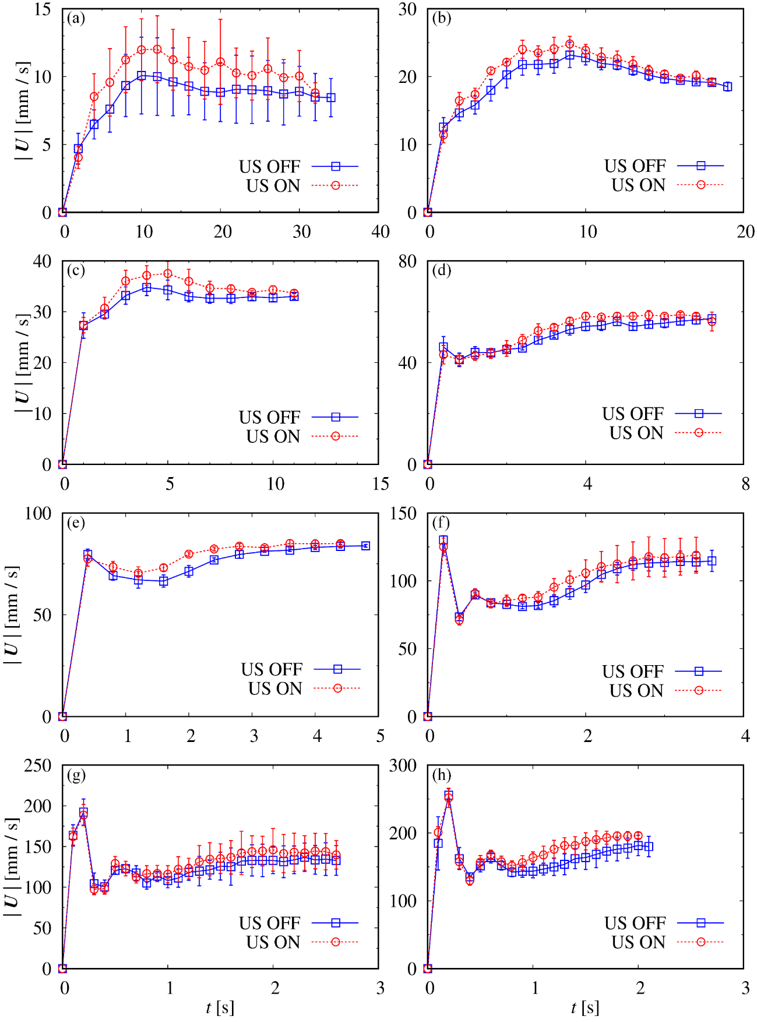
\includegraphics[width=13cm,clip]{5-Results/iwamuro-fall.png}
        \caption{Speed of a falling sphere in diameter of (a) 3 mm, (b) 4 mm, (c) 5 mm, (d) 6 mm, (e) 7 mm, (f) 8 mm, (g) 9 mm, (h) 10 mm in 1.0 wt.\% PAA solution with ultrasound fixed frequency at 27.4 kHz and $\Delta \bar{P} \approx$ 180 kPa\cite{ref:8}.}
        \label{fig:iwamuro-fall}
    \end{center}
\end{figure}

\begin{figure}[ht]
    \begin{center}
        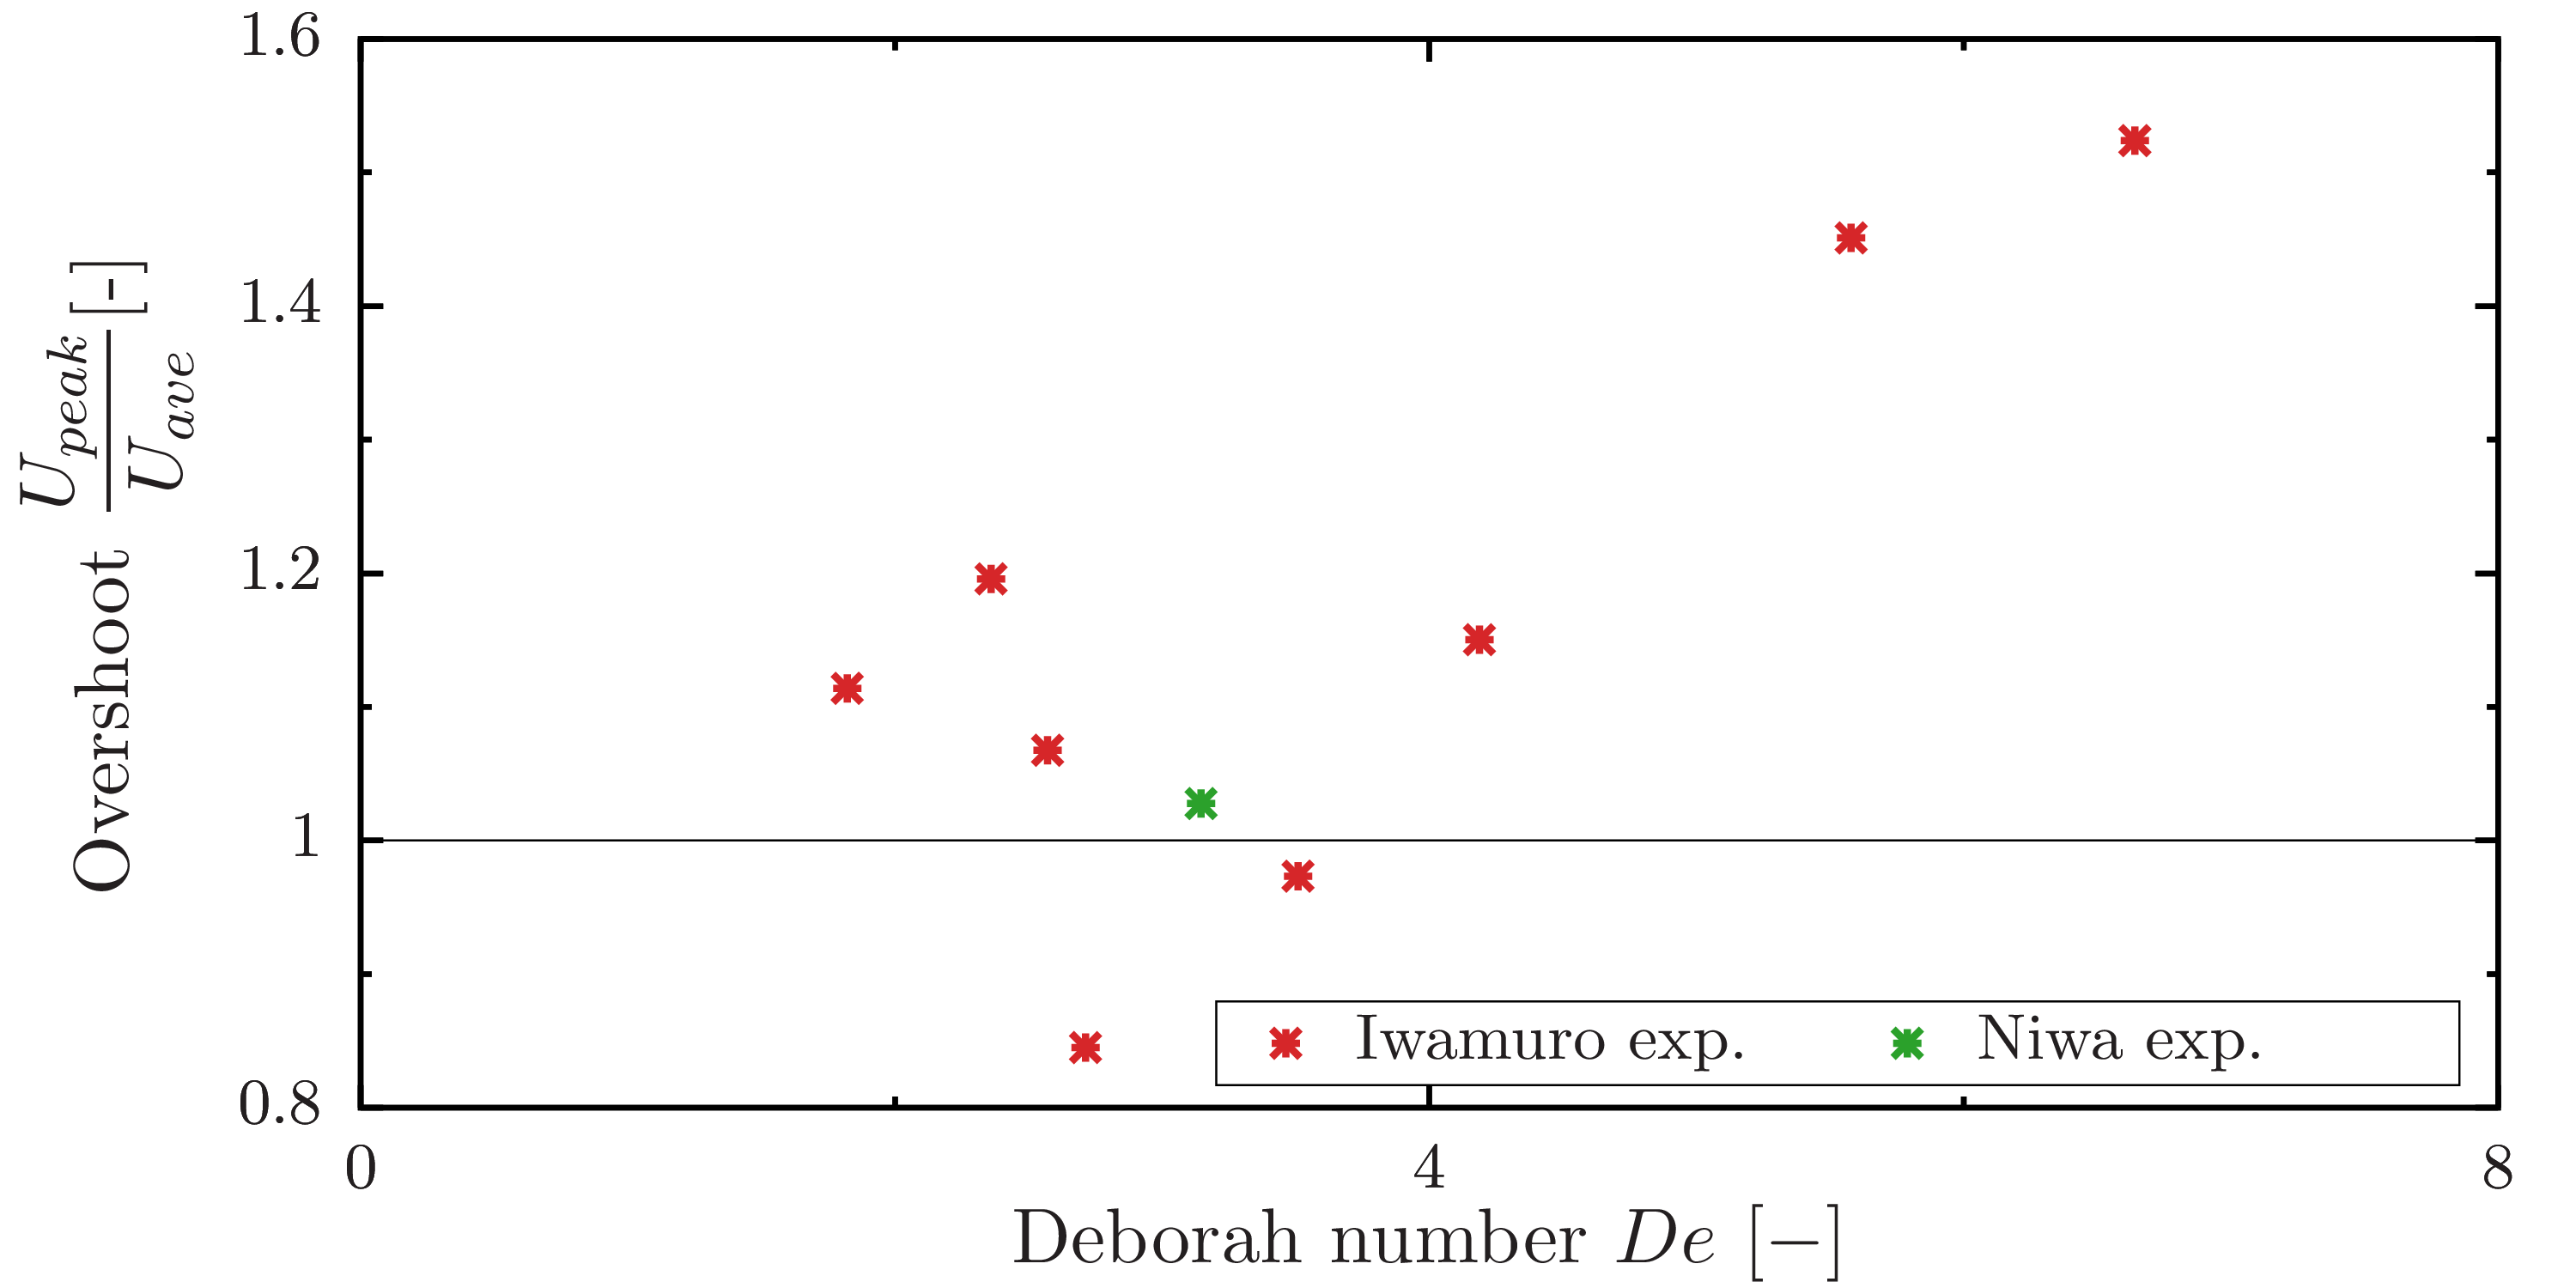
\includegraphics[width=15cm,clip]{5-Results/De-overshoot.png}
        \caption{Relationship between overshoot $U_{peak}/U_{ave}$ and Deborah number $De$ for falling spheres.}
        \label{fig:De-overshoot}
    \end{center}
\end{figure}

\clearpage

\subsection{実験装置改良に伴う初速へ影響}

前節にて,実験装置の改良によってピーク速度が減少し,$De$が小さくなったことによってオーバーシュートが小さくなったことを示した.本節において,電磁石を用いて把持した場合,ピーク速度が大きくなった理由に関して考察を行う.電磁石を用いて球を把持した場合,電磁石へ落下方向に力を与えて落下を開始させている.この時,微小ではあるが落下開始時に初速が存在する.一方で真空ポンプを用いて球を把持した場合,吸着パッドを大気圧にすると球は落下する.この場合,球に力が加わらないため,初速は存在しない.このように初速の有無がオーバーシュートの変化に大きく関与していると考えられる.

初速の有無が与える影響に関して調査するため,真空ポンプを用いて球中心が液面より高さ$H=$5mmとなる地点で把持し,そこから球を落下させた.その結果をFig.\ref{fig:h-5}に示す.縦軸は落下速度,横軸は初速ありの場合は液面に球中心が入ったときを0s,初速なしの場合は落下開始時刻を0sとした時刻である.この条件において,初速は313[mm/s]となる.ピーク速度は440[mm/s]となり,初速を超えて加速した.これは初速と重力による加速が,粘性抵抗や浮力よりも大きく,弾性は遅れて発生するため,初速を超えて加速したと考えられる.

Iwamuro\cite{ref:9}の$a =$5[mm]における初速を推定する.この結果において,0.1sの時185[mm/s]であった.球の初速を$U_0$とすると,$U_0$の取りうる値の範囲は,0$\leqq U_0 \leqq$185[mm/s]となる.一方で,ピーク速度は256[mm/s]となり,オーバーシュートが見られた.これは,先述の初速を与えた結果と同様に弾性による影響が生じる前に初速や重力によって加速したためだと考えられる.

また,真空ポンプを用いた落下実験(niwa exp.)の$De$数は,先行研究の結果において球半径$3<a<3.5$[mm]の間における$De$数に相当した.電磁石を用いて把持した実験において,この球径においてオーバーシュートはあまり見られなかった.真空ポンプを用いた落下実験の場合,$De$数が小さくなった原因であるが,初速が存在しないため急激な速度変化とならず,ピーク速度$U_{peak}$が小さくなったためと考えられる.

よって,電磁石を用いて球を把持した場合は初速による影響がオーバーシュートとして現れるが,真空ポンプを用いて球を把持した場合は初速が非常に小さいためその影響を受けないということが分かった.

\begin{figure}[ht]
    \begin{center}
        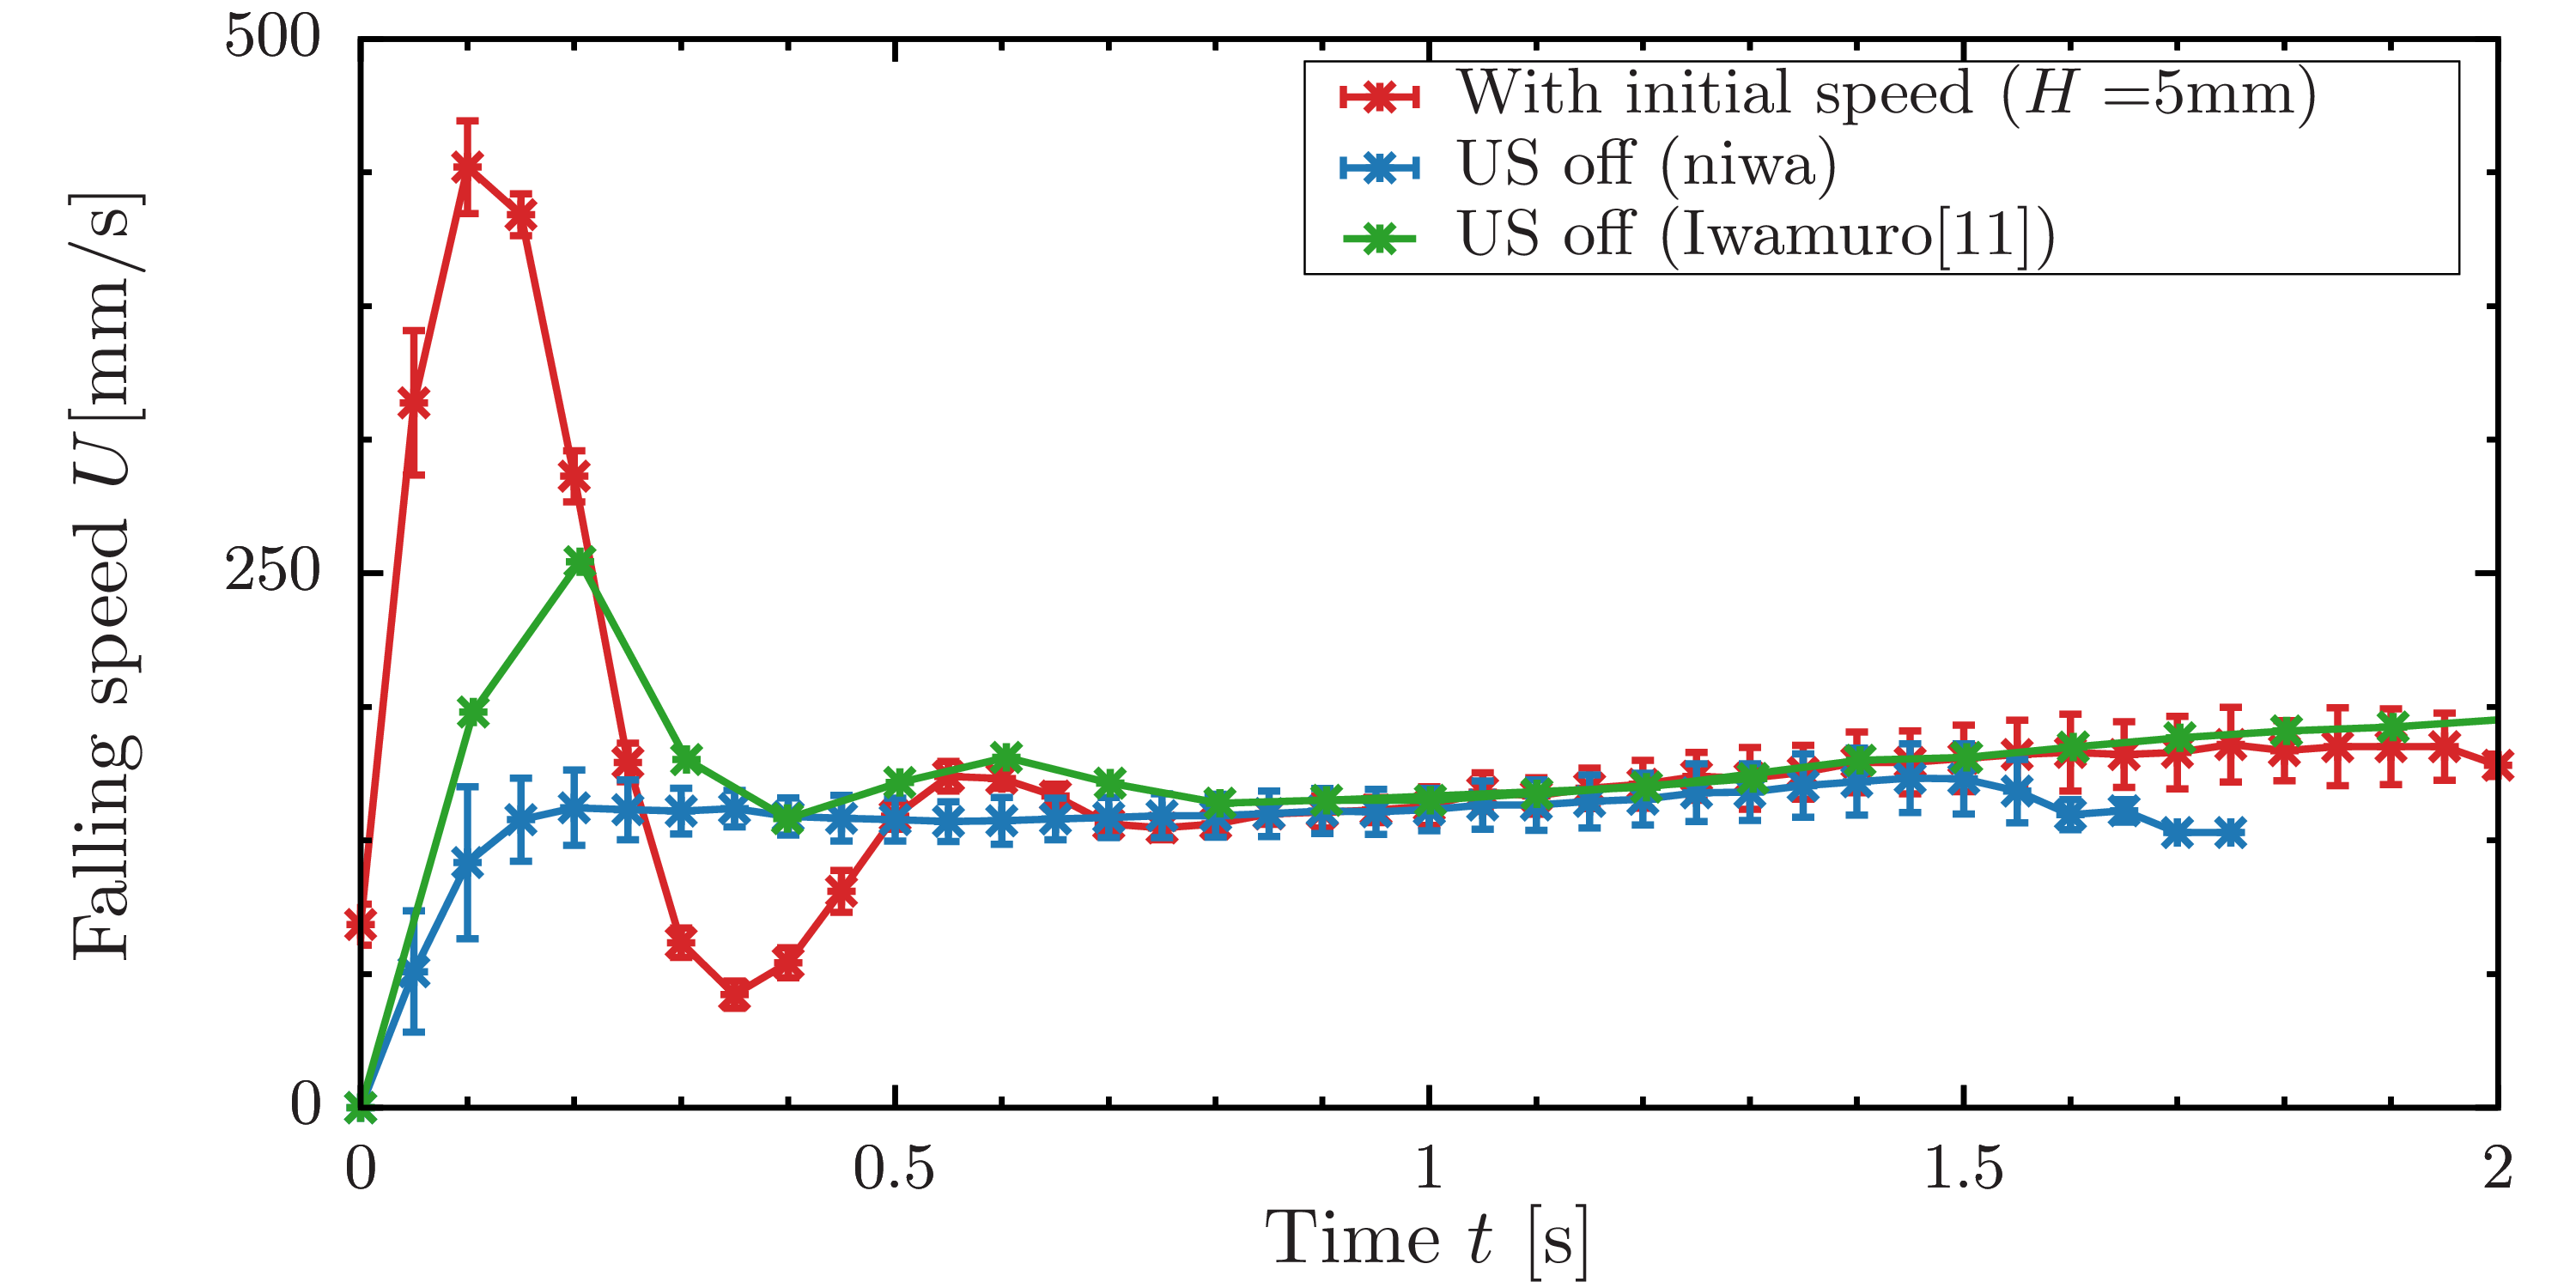
\includegraphics[width=15cm,clip]{5-Results/h-5.png}
        \caption{Falling speed of a sphere in 1wt.\% PAA solution falling with initial speed.}
        \label{fig:h-5}
    \end{center}
\end{figure}